% !TeX spellcheck = cs_CZ
{\tikzset{external/prefix={tikz/FYZI/}}
 \tikzset{external/figure name/.add={ch40_}{}}
%=========================== Kapitola: Principy statistické mechaniky =============================
\chapter{Principy statistické mechaniky}\label{fyz:IchapXL}
\minitoc
  \section{Exponenciální atmosféra}\label{fyz:IchapXLsecI}

    \begin{figure}[ht!] %\ref{fyz_fig344}
      \centering
      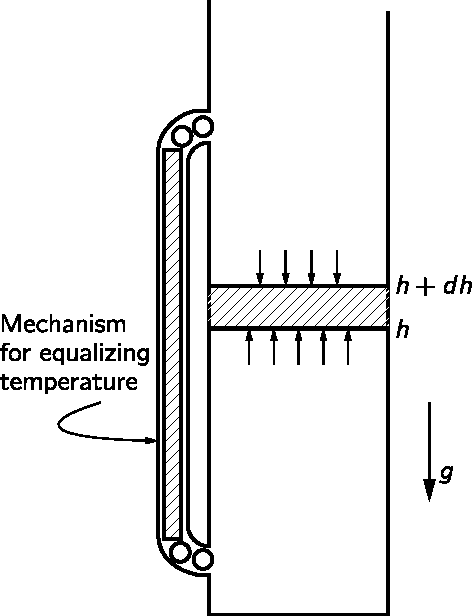
\includegraphics[width=0.7\linewidth]{fyz_fig344.pdf}
      \caption{Tlak ve výšce \(h\) musí převyšovat tlak ve výšce \(h+\dd{h}\) o tíhu plynu 
               nacházejícího se v takto ohraničené vrstvě
               (\cite[s.~540]{Feynman01})}
      \label{fyz_fig344}
    \end{figure}

    \begin{figure}[ht!] %\ref{fyz_fig345}
      \centering
      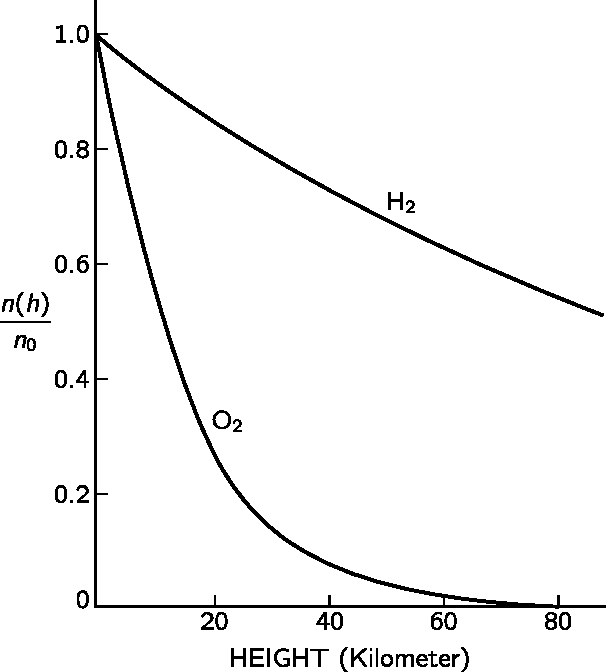
\includegraphics[width=0.7\linewidth]{fyz_fig345.pdf}
      \caption{Normovaná hustota jako funkce výšky v gravitačním poli Země - pro kyslík a vodík při 
               konstantní teplotě
               (\cite[s.~541]{Feynman01})}
      \label{fyz_fig345}
    \end{figure}
    
  \section{Boltzmannův zákon}\label{fyz:IchapXLsecII}
  \section{Vypařování kapaliny}\label{fyz:IchapXLsecIII}
  \section{Rozdělení molekul podle rychlosti}\label{fyz:IchapXLsecIV}
  \section{Měrná tepelná kapacita plynů}\label{fyz:IchapXLsecV}
  \section{Selhání klasické fyziky}\label{fyz:IchapXLsecVI}
  \section{Příklady a cvičení}\label{fyz:IchapXLsecVII}
  
    \begin{figure}[ht!] %\ref{fyz_fig346}
      \centering
      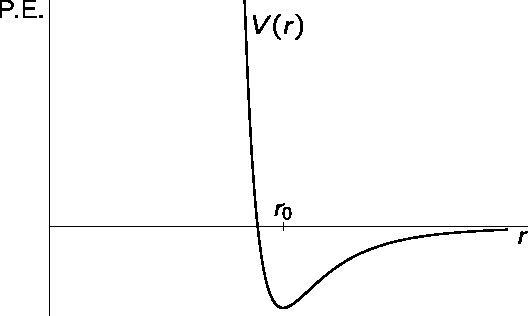
\includegraphics[width=0.7\linewidth]{fyz_fig346.pdf}
      \caption{Graf závislosti potenciální energie dvou molekul na jejich vzdálenosti
               (\cite[s.~543]{Feynman01})}
      \label{fyz_fig346}
    \end{figure}

    \begin{figure}[ht!] %\ref{fyz_fig347}
      \centering
      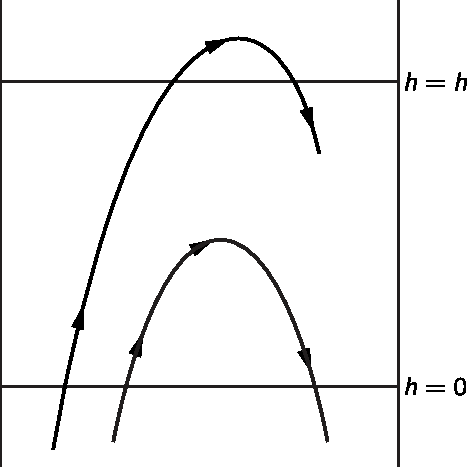
\includegraphics[width=0.7\linewidth]{fyz_fig347.pdf}
      \caption{Výšky \(h\) dosahují jen ty molekuly, které se ve výšce \(h=0\) pohybovaly 
               dostatečně rychle
               (\cite[s.~545]{Feynman01})}
      \label{fyz_fig347}
    \end{figure}

    \begin{figure}[ht!] %\ref{fyz_fig348}
      \centering
      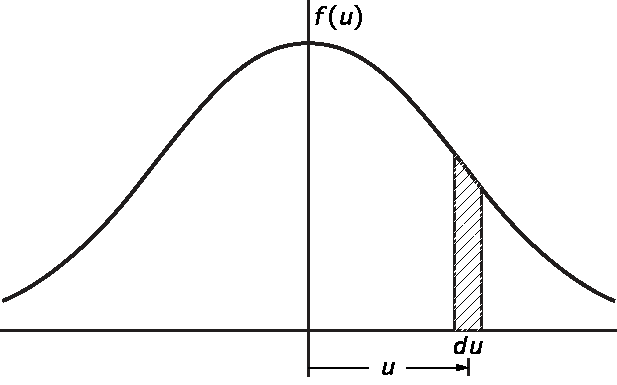
\includegraphics[width=0.7\linewidth]{fyz_fig348.pdf}
      \caption{Distribuční (rozdělovací) funkce rychlostí. Vyšrafovaná plocha představuje 
               \(f(u)\dd{u}\), tj. relativní počet částic s rychlostmi z intervalu šířky \(\dd{u}\) 
               v okolí \(u\)
               (\cite[s.~525]{Feynman01})}
      \label{fyz_fig348}
    \end{figure}

    \begin{figure}[ht!] %\ref{fyz_fig349}
      \centering
      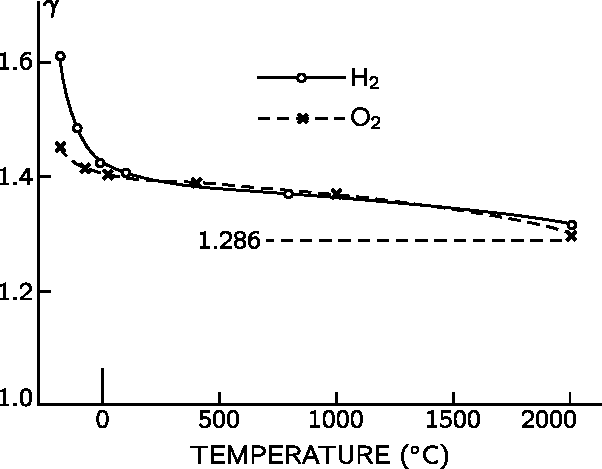
\includegraphics[width=0.7\linewidth]{fyz_fig349.pdf}
      \caption{Experimentální hodnoty \(\gamma\) jako funkce teploty pro vodík a kyslík. Klasciká 
               teorie předopovídá \(\gamma =\num{1.286}\) nezávisle na teplotě. 
               (\cite[s.~525]{Feynman01})}
      \label{fyz_fig349}
    \end{figure}

} %tikzset
%---------------------------------------------------------------------------------------------------
\printbibliography[title={Seznam literatury}, heading=subbibliography]
\addcontentsline{toc}{section}{Seznam literatury}